% cap2.tex

\chapter{Marco Teórico}
\label{c2} 


\section{\textit{Cap and Trade} y otros sistemas actuales}\label{c22}
%Agregar desde segundo párrafo de la Revision bibliográfica del hito 1

En el contexto de la generación de energía, el medio ambiente es directamente afectado por la tecnologías utilizadas. Con el fin de generar energía, se necesita de la combustión de un material, el aprovechamiento mecánico de una energía natural externa u otra fuente como energía nuclear. Estos sistemas provocan, en distintos niveles y formas, efectos en el medio ambiente. Particularmente, las termoeléctricas son consideradas como las que más emisiones de dióxido de carbono producen.
\vspace{2.5mm}

La última importante mención por parte del Gobierno de Chile, sobre su plan para combatir esta situación, es la propuesta climática a largo plazo que el Ministerio del Medio Ambiente de Chile presentó en la COP26 el mes de octubre de 2021 (\citeB{gobierno_de_chile_estrategia_2021}). En ella, se proponen medidas drásticas para combatir las emisiones por medio de una propuesta específica en la Sección de generación de energía. En ella, se presenta un presupuesto límite de emisión de carbono para los generadores de energía. Sin  embargo, en contraste, no se incluye un mecanismo o plan específico de cómo las empresas generadoras lograrán esto y de qué forma se llevará a cabo la supervisión de esta meta.
\vspace{2.5mm}

Desde que se identificó al efecto invernadero como un problema, varios países han comenzado a intervenir, directa o indirectamente, en las industrias que más aportan al efecto. 
\vspace{2.5mm}

Por un lado, el impuesto al carbono o impuesto a emisiones de $CO_2$ consiste en un costo adicional para la generación de electricidad con energías no renovables. El impuesto es cobrado por cada tonelada emitida de este compuesto. \citeB{asen_carbon_2021} menciona que Finlandia, en 1990, fue el primer país en implementarlo y desde ese momento 18 otros países del continente y muchos otros en el planeta lo fueron aplicando a distintos valores por tonelada emitida.
\vspace{2.5mm}

Por otro lado, existen los modelos de \textit{cap and trade}, concepto creado por Thomas Crocker. Según \citeB{hanemann_cap-and-trade_2010} este consiste en que un ente regulador determina capacidades máximas de contaminación por emisiones a las empresas de la industria eléctrica. Estos emisores son regulados y se les asignan permisos con determinados márgenes, por lo tanto, si superan la capacidad permitida, deben pagar penalizaciones.
\vspace{2.5mm}

En un contexto en el cual se busca cumplir con promesas por país para lograr el acuerdo de París (no aumentar la temperatura global en más de 2°C para fines del siglo), un modelo de \textit{cap and trade} es el que se presenta como una mejor opción. Esto se debe a que permite establecer, inicialmente, capacidades límites por industria o por país. Entonces, la regulación de un máximo de contaminación es más factible con un modelo que limite el contaminante de cada agente contaminador. Sin embargo, el problema radica en que cada tipo de \textit{cap and trade} implementado puede afectar en distintas formas la industria, las empresas involucradas y la demanda energética. Por un lado, se puede lograr minimizar emisiones gracias a la reducción en la generación y, por otro lado, se puede lograr aumentar la cantidad de empresas generadoras con energías renovables.
\vspace{2.5mm}

\citeB{chen_renewable_2021} prueban que aplicar un mecanismo de \textit{cap and trade} es mucho más efectivo en reducir las emisiones de carbono y en incentivar la inversión en energías renovables en comparación con no implementar ningún mecanismo de \textit{cap and trade}. Los autores estudian 3 escenarios aplicados a una empresa monopólica. Los escenarios son los siguientes: sin mecanismo de cap-and-trade (NM), con \textit{cap and trade} de regla Grandfathering (GM)\footnote{Mecanismo en el cuál una cuota total de carbono emitido  se determina para cada empresa según sus emisiones pasadas. \cite{chen_renewable_2021}} y mecanismo de \textit{cap and trade} con regla Benchmarking (BM).\footnote{El gobierno determina una cuota por unidad de carbono emitido.\cite{chen_renewable_2021}} 
\vspace{2.5mm}

El estudio concluye que al implementar mecanismos siempre existirá una mejora en el área de inversión en energías no convencionales o en la reducción en emisiones de carbono. No obstante también concluyen que un aumento en la inversión en energías renovables no reduce necesariamente las emisiones de carbono totales, debido a que esta inversión puede ser resultado o respuesta únicamente del aumento en generación y no un reemplazo de generación con un nuevo tipo de origen. Entonces, además demuestran que la implementación de BM incentiva más este tipo de inversión y, por el contrario con GM se produce menos emisiones de carbono. De esto, es importante destacar que el tipo de mecanismo de \textit{cap and trade} afecta en gran medida el resultado, entonces se debe construir un modelo que logre las promesas de contaminación propuestas y no implementar cualquier mecanismo. 
\vspace{2.5mm}

\citeB{wang_impact_2021} se focalizan en el efecto que las implementaciones de los mecanismos \textit{Benchmarking} y \textit{Grandfathering} tienen en las cadenas de suministro de las empresas. Se evalúan cómo los modelos de financiamiento Bank Credit Financing (BCF)\footnote{El banco otorga un crédito con la necesidad de que se aplique a bajar emisiones de la empresa prestataria.\cite{wang_impact_2021}} y Trade Credit Financing (TCF)\footnote{Crédito que permite atrasar el pago del manufacturero al proveedor.\cite{wang_impact_2021}}, en conjunto con BM y GM, afectan las cadenas de suministro de las empresas y de que forma estas se comportan. Se observa el comportamiento de un productor y su proveedor. Finalmente, se concluye que sin importar el mecanismo de \textit{cap and trade}, los productores o fabricantes siempre prefieren BCF, mientras que los proveedores se inclinan por TCF. Además, el tipo de mecanismo que sea conveniente para el productor dependerá principalmente de sus emisiones históricas.
\vspace{2.5mm}

En estos estudios, se reconoce la importancia de la implementación del tipo de modelo y de cómo el presupuesto de carbono total puede afectar al mercado. A pesar de esto, el mismo creador del modelo de \textit{cap and trade} mencionó, en el año 2009, ``Soy escéptico de que un modelo de cap-and-trade sea la forma más eficaz de regular el carbono'',\footnote{{\scriptsize \url{https://www.businessinsider.com/inventor-of-cap-and-trade-says-a-carbon-tax-is-better-2009-8}}} debido a que él concluía que era difícil predecir cómo este modelo afectaría al mercado de generación en el futuro, además, si no se tiene un ente regulador, que fiscalice las emisiones continuamente y establezca las capacidades de forma apropiada, un modelo únicamente con impuesto a la emisión parece ser más eficaz. Entonces, un modelo que se pueda regular solo, en el cual exista incentivo en la disminución de emisión, en el que las empresas generadoras tengan más de una oportunidad para cambiar sus inversiones en capacidad y permisos y que este cambio signifique un beneficio para las empresas, sería un camino apropiado para un modelo de \textit{cap and trade} efectivo. Los autores \citeB{amigo_two_2021} proponen un sistema con estas características.


\section{Problemas de equilibrio en capacidad} \label{c21}

Con el fin de interpretar la toma de decisiones de los agentes en cualquier sistema, es necesario modelar los mecanismos en los cuales están involucrados los diferentes actores. Los modelos de optimización bien diseñados orientan la toma de decisiones en base a variables que pueden describir la estrategia de un agente. Estas variables son interpretación de qué decisiones deben tomar los agentes involucrados mientras estos tengan el poder de cambiarlos. 
\vspace{2.5mm}

Un modelo bien estructurado, con restricciones basadas en la teoría económica, puede, por una parte, significar un cambio operacional y táctico para una empresa o actor que busca optimizar algún problema. Por otra parte, un modelo puede mostrar el comportamiento esperado de un mercado.
\vspace{2.5mm}

Los modelos de equilibrio son aquellos que representan un problema donde los tomadores de decisión (representados por conjuntos de variables y funciones objetivos en el modelo) cumplen con una optimalidad individual y restricciones de equilibrio asociadas a sus decisiones que relacionan las acciones óptimas de todos los agentes involucrados.
\vspace{2.5mm}

Estos modelos, por ejemplo, representan las estrategias de varios agentes involucrados para el abastecimiento de una demanda de mercado. 
\vspace{2.5mm}

Esta memoria se focaliza en los modelos de equilibrio en capacidad, relacionados con el mercado de generación eléctrica. En estos, por una parte, presentan un equilibrio entre la demanda de energía de los consumidores y la oferta de los productores y, por otra parte, un equilibrio entre la capacidad instalada de los productores y los permisos para emitir contaminantes. Este problema se formula como la minimización anual de inversión en las plantas generadoras de energía.
\vspace{2.5mm}

Los modelos de equilibrio en capacidad han sido estudiados por \citeB{ehrenmann_generation_2011}, \citeB{d__aertrycke_risk_2017}, \citeB{gabriel_complementarity_2012}, \citeB{ralph_risk_2015}, entre otros.
\vspace{2.5mm}

A continuación, en base al trabajo de \citeB{d__aertrycke_risk_2017}, se explica un problema de equilibrio en capacidad con riesgo asociado de dos etapas y uno de riesgo neutral.

\subsection{Problema de equilibrio en capacidad con riesgo asociado (\textit{risky design equilibrium problem}) y modelos de dos etapas}

En este tipo de problemas, existe una variable o vector de variables de diseño denotada como  $x \in \mathbb{R}^{n}$, la cual describe la inversión en activos riesgosos tales como plantas de producción de energía que llevan consigo poderes de producción determinados y proporcionales al grado de inversión en mercados con incertidumbre de demanda.
\vspace{2.5mm}

Es importante entender que estos son problemas de optimización estocásticos. Es decir, existe aleatoriedad respecto a los parámetros de entrada. En este caso, la aleatoriedad se ve reflejada en los escenarios estocásticos posibles con $w \in \Omega:=\{1,...,K\}$. Entonces, por ejemplo, existen costos $C^{w}$ que corresponden a cada escenario $w$. 
\vspace{2.5mm}

La probabilidad de ocurrencia de cada escenario depende de una distribución de probabilidad $\Theta$, la cuál debe ser definida en el problema estudiado y una de sus aplicaciones es con la notación de valor esperado $E_{\Theta}[Z]$. Esta corresponde a la suma ponderada con una probabilidad de ocurrencia para una realización particular $z_{w}$ de la variable aleatoria $Z$ . En otras palabras, $E_{\Theta}[Z]$ es una suma ponderada de los valores de una variable en todos los escenarios multiplicados por la probabilidad de ocurrencia de cada escenario. En el Anexo \ref{ej:sumapond} se presenta un ejemplo de lo anterior.
\vspace{2.5mm}

Generalmente, estos modelos, tienen dos etapas de decisión $s\in\{0,1\}$ para los agentes diseñados en el problema. En la primera etapa $s=0$, el productor (monopolio) o grupo de productores (mercado competitivo) decide su inversión en capacidad $x$. Luego, en la segunda etapa $s=1$, se decide la producción $Y$ (si existe más de un escenario de ocurrencia, estos presentan distintas demandas o costos). Es decir, la variable de producción también puede depender del escenario $w$, teniendo $Y_{w}$ para cada uno).
\vspace{2.5mm}

 \citeB{d__aertrycke_risk_2017}, identifican estos problemas como aquellos en los que existe una función $f$ convexa y continua, $g$ convexa y continua en los que para cada $x$:

\begin{align}
\min f(x,y)\quad\text{sujeta a}\quad g(x,y)\leq 0
\end{align}


Este problema de optimización busca minimizar los costos asociados al problema y $g(x,y)$ puede ser una o un grupo de restricciones tecnológicas o de equilibrio del sistema.\footnote{Ver página 11 de \citeB{d__aertrycke_risk_2017}.} 
\vspace{2.5mm}

Con el fin de contrarrestar los costos asociados a escenarios con incertidumbre, por ejemplo, sub o sobre inversión, según cada escenario, cada agente $i$ se dota de una medida de riesgo $r_{i}$ que mide el costo de la incertidumbre respecto de una variable incierta (variable aleatoria o estocástica). Para mitigar ese costo por riesgo, el agente puede decidir qué productos financieros $W_i\in\mathbb{R}^K$ elegir para compensar el riesgo de incertidumbre en cada escenario. Estos productos tienen un precio asociado $P^{r}[W_i]$. Este precio es determinado por la condición de que todos los productos financieros deben balancearse y, suponiendo que $N>0$ agentes componen el mercado, lograr que:

\begin{eqnarray}
\sum_{i=1}^{N}W_{i} &=& 0\label{eq:fin-eq}    
\end{eqnarray}

En otras palabras, si un agente necesita un contrato o producto financiero que asegure un determinado valor en el escenario $w$, la condición de equilibrio o balance (ecuación \ref{eq:fin-eq}) anterior asegura que existe otro agente dispuesto a entregar (o prestar) ese valor. Esa entrega o préstamo tiene un valor determinado endógenamente por $P^r$.\vspace{2.5mm}

En cada una de las dos etapas de este sistema, existen importantes consideraciones.
\vspace{2.5mm}

En la primera etapa, la empresa generadora toma una decisión de inversión en capacidad $x$ que acotará la máxima producción. 
\vspace{2.5mm}

En la segunda etapa, se conoce la demanda del periodo y la empresa generadora minimiza sus costos. La producción es $Y_{w}$ para el escenario $w$ y se vende la energía a un precio $P_{w}\geq 0$ y costo $C_{w}(Y_{w})$. En cada escenario $w$, la empresa buscará maximizar las utilidades o minimizar los costos de operación y, al mismo tiempo, el demandante buscará maximizar sus utilidades de demanda $Q_{w}$ al comprar la energía al precio $P_{w}$.

\subsection{Tratamiento del riesgo}

La forma en cómo se valora el riesgo usualmente se ha clasificado entre aversos, neutrales y amantes. Dicha tipología tiene directa relación con la curvatura de la función objetivo que evalúa un valor incierto. La aversión al riesgo se representa mediante la concavidad, la neutralidad con funciones lineales como un valor esperado y el gusto por riesgo con convexidad. En lo que sigue nos centraremos en el caso estándar de riesgo neutralidad como supuesto simplificador.

Este es el caso en el que todos los agentes involucrados en el problema conocen sus costos estocásticos del problema con la probabilidad $\Theta$ anteriormente explicada de cada escenario $w$. Esto significa que aquellos costos asociados a la producción respetan esta probabilidad, sin embargo los costos de inversión en capacidad no son estocásticos, por lo tanto, no son afectados directamente por esta. En el caso neutral al riesgo, existe solamente el riesgo en inversión de capacidad, pero no un riesgo de compra de activos financieros ya que los agentes, en este caso, son neutrales al riesgo de intercambio o compra de activos financieros. 
\vspace{2.5mm}

Como se mencionó anteriormente, este estudio explora la aplicación de estos modelos en el mercado de empresas generadoras de electricidad, en que existen dos tipos de agentes: empresas generadoras únicamente de electricidad y demandantes de la energía producida. Este es un caso que puede ser tomado como de mercado competitivo, en el que las empresas no actúan estratégicamente para influenciar los precios. 
\vspace{2.5mm}

Bajo estas circunstancias, se tiene que este es un problema competitivo de equilibrio en capacidad riesgo neutral si es que existe un grupo de variables, $x_{1}$ para la inversión en capacidad del primer generador, $Y$ para la cantidad ofertada de electricidad para cada escenario $\omega$), $x_{2}$ para la inversión en capacidad del segundo generador, y $Q$ para la demanda energética. El problema debe resolver lo siguiente: 

\begin{align}
 \text{min } I_{1}(x_{1})+ I_{2}(x_{2})+E_{\Theta}[C_{w}(Y_{w}-U_{w}(Q_{w})] \label{foejemplomaere}
\end{align}

sujeto a

\begin{align}
 x_{1} \in X_{1} ,x_{2} \in X_{2}\label{res1ejemplomaere}\\
A_{1w}x_{1}+B_{1w}Y_{w}+b_{1w} \le 0 \label{res2ejemplomaere}\\
A_{2w}x_{2}+B_{2w}Y_{w}+b_{2w} \le 0 \label{res3ejemplomaere}\\
Q_{w}\le e^{\tau}Y_{w}\text{  }\text{ para todo w}\label{res4ejemplomaere}
\end{align}

Modelo en el cuál, la función objetivo \ref{foejemplomaere} minimiza el negativo de utilidad. La restricción \ref{res1ejemplomaere} acota la elección de estrategia de inversión para cada agente según su \textit{set} de estrategias $X_i$. Las restricciones \ref{res2ejemplomaere} y \ref{res3ejemplomaere} acotan los recursos de cada agente según su capacidad de inversión y oferta. La última restricción \ref{res4ejemplomaere} solicita que la demanda se debe abastecer completamente.



\section{MCP y Programación modelos de equilibrio}

\subsection{Resolución Problemas de equilibrio mediante MCP}\label{descripcionkkt}

La mayoría de los estudios sobre modelos de equilibrio, mencionados anteriormente, explican que la mejor forma de resolver los problemas de este tipo, en especial aquellos con gran cantidad de variables o aquellos no lineales, es transformarlos en problemas de complementaridad mixta o \textit{Mixed Complementarity Problems} (MCP por sus siglas en inglés, ver objetivo específico b) en el capítulo introductorio).
\vspace{2.5mm}

\citeB{gabriel_complementarity_2012} explican que para realizar esto, es necesario estructurar el problema de equilibrio de la siguiente forma:

\begin{align}
    \min_{x} & \quad f(x) \label{foej1}\\ 
    \textrm{s.a.} \nonumber\\
    g_{i}(x) \leq 0 ,\quad & i=1,2,...,n  &(\eta_{i}) \label{resej1} 
\end{align}

Con $f(x)$ función objetivo,  $g_{i}(x):\mathbb{R}^n \rightarrow \mathbb{R}$ restricciones y $\eta_i$ los multiplicadores de Lagrange asociados. 
\vspace{2.5mm}

Puede suceder que las restricciones son con sentido inverso y para eso solo basta con multiplicar la restricción \ref{resej1} por $-1$ y así obtener el sistema de ecuaciones deseado. Si la función objetivo \ref{foej1} es una maximización, basta con multiplicarle $-1$ a la función para convertirla en minimización.
\vspace{2.5mm}

Luego, se debe calcular el Lagrangeano de este problema con las variables duales de cada restricción ($\eta_{i}$ en \ref{resej1}) de la siguiente forma:

\begin{align}
    \mathcal{L}=f(x) +  \sum_{i=1}^{n}\eta_{i}g_{i}(x)\label{lagraneanoex}
\end{align}

Finalmente, se puede encontrar un valor óptimo para $x$, en que se cumplan las siguientes condiciones de \textit{Karush-Kuhn-Tucker} (KKT). La primera condición \ref{condicion1}, restringe que el gradiente respecto a la variable $x$ del Lagrangeano en \ref{lagraneanoex} debe ser 0 (estacionariedad). La segunda y tercera condición \ref{condicion2}, \ref{condicion3}, establecen la no negatividad de las restricciones (factibilidad). La última condición \ref{condicion4} establece la complementariedad entre la restricción y su variable dual respectiva\footnote{\ref{condicion2},\ref{condicion3},\ref{condicion4} pueden ser resumidas en una sola condición como: $0\leq\eta_{i}\perp g_{i}(x)\leq 0$}. 

\begin{align}
    0 = \nabla f(x) + \sum_{i=1}^{n} \eta_{i}\nabla g_{i}(x) \label{condicion1}\\
    -g_{i}(x) \geq 0 &, & i=1,2,...,n  \label{condicion2}\\
    \eta_{i} \geq 0 &, & i=1,2,...,n \label{condicion3}\\
    -g_{i}(x)\cdot \eta_{i} = 0 &, & i=1,2,...,n \label{condicion4}
\end{align}

\subsection{Programación de los modelos de equilibrio}\label{explisolvers}

A pesar de que existen diversos lenguajes de programación que soportan optimización de modelos y muchos de estos contienen librerías especializadas para encontrar estas soluciones, la utilización de programas que soporten problemas no lineales NLP (por las siglas \emph{Non Linear Problems} en inglés) son más convenientes de aprender. Esta sub-sección explica el método de cómputo de modelos de equilibrio NLP en \textit{pyscipopt} (librería soportada por Python), GAMS, MCP específico en GAMS y Gurobi(\textit{solver} aplicado en lenguage Julia).

\subsubsection{\textit{Pyscipopt}}

SCIP es una librería de código abierto para distintos programas. En su página web oficial, se solicita citar los siguientes 2 artículos \citeB{perron_constraint_2008}
y \citeB{achterberg_scip_2009} al utilizar el \textit{solver} para un trabajo. 
\vspace{2.5mm}

\textit{Pyscipopt} es la interfaz desde python a la \textit{SCIP Optimization Suite}. La ventaja de este \textit{solver}, además de entregar resultados certeros de modelos no lineales, es que presenta la posibilidad de incluir sumatorias propias para definir las restricciones con mayor facilidad y su notación simplifica la posibilidad de incluir variables y de utilizar las funciones usuales de Python sin el cuidado de afectar la sintaxis del solver.
\vspace{2.5mm}

Con el fin de utilizar este programa es necesario instalar ciertas librerías antes de \textit{pyscipopt}. La forma recomendada es utilizar Google Colab como interfaz de Python.\footnote{Ver \url{https://research.google.com/colaboratory/faq.html}} Una vez en un archivo Colab, es necesario agregar las siguientes líneas de código:

\begin{footnotesize}
\begin{lstlisting}[language=Python]
!pip install -q condacolab
import condacolab            
condacolab.install()
!conda install --channel conda-forge pyscipopt
\end{lstlisting}
\end{footnotesize}

% Waiting answer here:
% https://github.com/gpoore/minted/issues/233
%\begin{listing}[!ht]
%\begin{minted}{c}
%#include <stdio.h>
%int main() {
%   printf("Hello, World!"); /*printf() outputs the quoted string*/
%   return 0;
%}
%\end{minted}
%\caption{Hello World in C}
%\label{listing:2}
%\end{listing}

Luego, la codificación del problema por resolver debe seguir la siguiente forma y condiciones:

\begin{enumerate}
    \item Comenzar el modelo: se debe escribir el comienzo del modelo o apertura de su diseño con el siguiente comando,
    
    \begin{footnotesize}
    \begin{lstlisting}[language=Python]
   modelo=Model()
   \end{lstlisting}
    \end{footnotesize}
   
   \item Definir las variables: es necesario definir todas las variables con la siguiente nomenclatura,
   
   \begin{footnotesize}
   \begin{lstlisting}[language=Python]
   x=modelo.addVar('x', vtype='C')  # C variables continuas 
   y=modelo.addVar('y', vtype='d') # d  variables discretas 
   \end{lstlisting}
   \end{footnotesize}
   
   \item Generar la función objetivo: se debe definir la función objetivo de manera directa o a partir de otra variable inventada. También se define si el problema es de minimización o maximización,
   
   \begin{footnotesize}
   \begin{lstlisting}[language=Python]
  modelo.setObjective(x+y, "minimize")
  \end{lstlisting}
   \end{footnotesize}
   
  \item Agregar las restricciones: hay que agregar las restricciones del modelo. La naturaleza de las variables se pueden agregar en la misma definición de las variables o como restricción,
  
  \begin{footnotesize}
  \begin{lstlisting}[language=Python]
  modelo.addCons(x>=y)
  modelo.addCons(x>=0)
  modelo.addCons(y>=0)
  \end{lstlisting}
  \end{footnotesize}
  
  
  \item  Resolver el problema: se agrega el comando para que el \textit{solver} optimice y así encuentre la mejor solución posible,
  
  \begin{footnotesize}
  \begin{lstlisting}[language=Python]
  modelo.optimize()
  \end{lstlisting}
  \end{footnotesize}
  
  \item  Llamar a las soluciones encontradas: Este paso no es necesario para resolver el problema, pero se necesita si se quieren visualizar las variables óptimas del problema,
  
  \begin{footnotesize}
  \begin{lstlisting}[language=Python]
  modelo.getVal(x)
  modelo.getObjVal()
  \end{lstlisting}
  \end{footnotesize}
  
\end{enumerate}

\subsubsection{GAMS}

Según lo mencionado en la página de \textit{GAMS Studio}\footnote{\url{https://www.gams.com/34/docs/UG_studio_tutorial.html}}, este es un programa que permite la programación e interfaz gráfica para ejecutar GAMS. Es un lenguaje de programación especializado en resolver modelos de optimización. Este sistema es específico para realizar modelamiento de múltiples tipos de modelos de optimización y con un gran número de herramientas para resolverlos. Una de las ventajas de utilizar \emph{GAMS Studio} es el detalle que se entrega luego de encontrada (o no) la solución a un problema de modelamiento. Este detalle muestra los valores óptimos encontrados de cada variables junto con sus intervalos de error posibles y entrega información detallada del computador en el cual se está trabajando. En caso de que el sistema no logre encontrar solución, este entregará esa información junto con los posibles errores del modelo. 
\vspace{2.5mm}

Con el fin de utilizar adecuadamente este programa, es importante entender el problema de optimización que se quiere modelar, considerando todas las restricciones del problema y definiendo todas las variables y parámetros. Con el fin de que no existan errores, es necesario utilizar los separadores “;” para cada línea de código y definir cuáles de estas corresponden a variables, escenarios, parámetros, ecuaciones, restricciones y función objetivo. 
\vspace{2.5mm}

Es importante entender para definir las restricciones que “=g=” significa “mayor que” , “=l=” significa “menor que” y “=e=” significa “igual que”.
\vspace{2.5mm}

Luego, la codificación del problema por resolver debe seguir la siguiente forma y condiciones:

\begin{enumerate}
   \item Definir las variables: es necesario definir las variables dependiendo de su naturaleza. Se emplea la siguiente nomenclatura,
   
   \begin{footnotesize}
    \begin{lstlisting}
  Positive Variable  x; % se define la variable positiva x
  Binary Variable y; % se define la variable binaria y
  Variable z; % se define la variable real z
   \end{lstlisting}
   \end{footnotesize}
  
   \item Se mencionan las ecuaciones del modelo: se deben mencionar todas las ecuaciones del modelo, 
   \begin{footnotesize}
   \begin{lstlisting}
 Equations
 fo funcion objetivo
 rest restriccion;
  \end{lstlisting}
   \end{footnotesize}
   
  \item Definir las ecuaciones: después de mencionarlas, hay que definir las ecuaciones del modelo,
  
  \begin{footnotesize}
   \begin{lstlisting}
  fo.. z=e=5x+2;
  rest.. x=g=0;
  \end{lstlisting}
  \end{footnotesize}
 
  
  \item  Definir el modelo y resolver: se define el modelo con las ecuaciones y variables antes definidas. Se llama al \textit{solver} con el cual resolverlo y se define si se debe minimizar o maximizar la función objetivo. 
  
  \begin{footnotesize}
  \begin{lstlisting}
  Model modelo
  /fo,rest/;
  solve modelo using minlp minimizing z;
  \end{lstlisting}
  \end{footnotesize}
  
  \end{enumerate}


\subsubsection{GAMS con MCP}

Programar un problema MCP en GAMS requiere seguir la misma nomenclatura y base mencionada en la subsección anterior. Con excepción del último punto de definición del modelo y de cómo llamar al \textit{solver}. 
\vspace{2.5mm}

Se requiere entender que para este estilo de resolución de MCP en \textit{GAMS} es necesario tener el problema transformado al formato de un MCP. Para esto, una de las opciones es realizarlo mediante las condiciones de KKT explicadas en \ref{descripcionkkt}. Una vez encontradas las condiciones, se debe utilizar cada una de las derivadas de primer orden del Lagraneano en \ref{condicion1} para despejar las variables duales del problema. Una vez realizado esto, y respetando que se cumpla \ref{condicion3}, se puede llamar al \textit{solver} para solucionar el problema. 
\vspace{2.5mm}

Por ejemplo, se asume que la derivada de primer orden \ref{condicion1} del lagrangeano de un problema de optimización es la siguiente (con $x$ variable primal y $\eta$ dual):

$$\frac{\partial \mathcal{L}}{\partial x}=0=x-\eta \leftrightarrow \eta=x$$

Luego, se define la ecuación $KKT$ que corresponde a la dual $\eta$:

\begin{footnotesize}
\begin{lstlisting}
  kkt.. x=g=0;
 \end{lstlisting}
\end{footnotesize}


Finalmente, asumiendo que no hay restricciones adicionales y que la variable x está definida previamente como una variable positiva, se define el modelo y se llama al \textit{solver} \textit{PATH} (para problemas MCP) de la siguiente forma:

\begin{footnotesize}
\begin{lstlisting}
  options mcp=path;
  model Modelo2
  /kkt.x/
  solve Modelo2 using mcp;
\end{lstlisting}
\end{footnotesize}


Es importante entender que la sección \textbf{/kkt.x/} es la que define la condición de complementariedad \ref{condicion4} del MCP. Siendo \textbf{/kkt.x/} el equivalente a  $kkt \perp x$. 

\subsubsection{Gurobi con \julia}\label{mtjulia}

Gurobi\footnote{Ver \url{https://www.gurobi.com/}} es un \textit{solver} de programación matemática con licencia académica gratis, reconocido por su rapidez y aplicabilidad en múltiples lenguajes de programación. En su instalación, se deben seguir las instrucciones presentes en la descarga luego de solicitar una licencia académica temporal. En su página oficial\footnote{Ver  \url{https://www.gurobi.com/products/gurobi-optimizer/}}, se encuentra todo lo necesario para adquirir la descarga y licencia, además se señalan las instrucciones de llamado para los distintos lenguajes que soportan Gurobi y distintos tutoriales para su aplicabilidad.
\vspace{2.5mm}

\julia\footnote{Ver \url{https://julialang.org/}. Un libro virtual está disponible en \url{https://introajulia.org/} está creado para aprender a utilizar Julia, incluso como primer lenguaje de programación.}, por su parte, es uno de los lenguajes de programación con mayor crecimiento en adopción por parte de programadores y en capacidad.\footnote{Ver {\tiny \url{ https://www.hpcwire.com/2021/01/13/julia-update-adoption-keeps-climbing-is-it-a-python-challenger/}}} Además, su diseño 'primitivo', pero intuitivo, lo convierte en uno de los lenguajes más eficientes. 
\vspace{2.5mm}

A continuación, se definen los pasos generales para programar un modelo de optimización en \julia, utilizando el \textit{solver} Gurobi. 


\begin{enumerate}
    \item Iterfaz Jupyter: Aunque este paso no es necesario (se puede programar con la consola de \julia), se recomienda utilizar la interfaz Jupyter\footnote{Ver \url{https://jupyter.org/}} para programar con \julia. Una vez en la terminal de \julia se debe escribir lo siguiente:
    
    \begin{footnotesize}
    \begin{lstlisting}
    using Pkg
    Pkg.activate(".") # Activate environment 
    #in current directory
    Pkg.instantiate() # Download all packages
    using WebIO
    WebIO.install_jupyter_nbextension() # Required for 
    #plotting in Jupyter notebooks

    using IJulia #Required for notebook
    notebook(dir=".") # Start the 
    #Jupyter notebook in this directory.
    \end{lstlisting}
    \end{footnotesize}
    
    Con esto, se debería abrir un \textit{notebook} de Jupyter en el navegador.
    
   \item Librerías: se llama a las librerías comúnmente utilizadas para optimizar de la siguiente forma:
   
   \begin{footnotesize}
   \begin{lstlisting}
   using JuMP,Gurobi
   \end{lstlisting}
   \end{footnotesize}
   
   \item Definir modelo: se define el modelo y el optimizador por utilizar para resolverlo:
   
   \begin{footnotesize}
   \begin{lstlisting}
   modelo=Model(Gurobi.Optimizer)
   \end{lstlisting}
   \end{footnotesize}
   
   \item Definir las variables: es necesario definir las variables según su naturaleza, con la siguiente nomenclatura,
   
   \begin{footnotesize}
   \begin{lstlisting}
  @variable(model, x>=0)  # Variable mayor a 0
  @variable(model, Y[i in 1:5]>=0) # 5 Variables 
  #Y mayores a 0
   \end{lstlisting}
   \end{footnotesize}
   
  \item Definir la función objetivo:
  
  \begin{footnotesize}
  \begin{lstlisting}
  @objective(modelo, Min, x + sum(Y[i] for i in 1:5)) 
   \end{lstlisting}
  \end{footnotesize}
  
  \item Definir las restricciones: se definen las restricciones del modelo.
  
  \begin{footnotesize}
  \begin{lstlisting}
  @constraint(model, demanda[i in 1:5], Y[i] == Q[i] )
  @constraint(model, capacidad[i in 1:5], Y[i]-x<=0.0)
  \end{lstlisting}
  \end{footnotesize}
  
  \item  Resolver: se llama al \textit{solver} para encontrar una solución.
  
  \begin{footnotesize}
   \begin{lstlisting}
  JuMP.optimize!(model)
  \end{lstlisting}
  \end{footnotesize}
 
  
  \item Visualizar resultados: Si se quieren ver los valores encontrados de alguna variable en específico, se debe realizar lo siguiente.
  
  \begin{footnotesize}
  \begin{lstlisting}
  println("Variable = ", JuMP.value.(Variable))
  \end{lstlisting}
  \end{footnotesize}
  
\end{enumerate}



\subsection{Resolución ejemplo 3.3.1 D'{}Aertrycke et al. (2017)}

Con el fin de aplicar lo expuesto en la sección \ref{explisolvers}, se lleva a cabo la resolución del problema 3.3.1, presente en la página 24 de \citeB{d__aertrycke_risk_2017}. Este es un problema competitivo de equilibrio en capacidad con riesgo neutral, el cual está relacionado con el tema central de este trabajo ya que modela la minimización de costos de generación de electricidad al suplir la demanda energética que esta abastece. 
\vspace{2.5mm}

\subsubsection{Explicación del Problema}

En este ejemplo, existe un productor que puede invertir únicamente en una tecnología de producción energética. La planta tiene un costo de capital anualizado $I=90 \frac{\textup{\euro}}{kW}$ y costo de operación $C=60 \frac{\textup{\euro}}{kW}$. El año se representa, para este caso, con duración en horas $\tau = 8760$ horas. 
\vspace{2.5mm}

$B = 1\textup{\euro}/MWh^2$ es un parámetro constante en todos lo escenarios $w \in W$ de la utilidad de abastecimiento de demanda $Q_w$: $U_w(Q_w) = A_wQ_w-\frac{B}{2}Q_w^2$. Mientras que el parámetro $A_w$ depende del escenario $w$ y tiene los siguientes valores para cada uno de ellos:

\begin{table}[H]
\centering
\begin{tabular}{|l|l|l|l|l|l|}
\hline
\textbf{w} & \textbf{1} & \textbf{2} & 3 & 4 & 5 \\ \hline
A {[$\frac{\textup{\euro}}{MWh}$]} & 300 & 350 & 400 & 450 & 500 \\ \hline
\end{tabular}
\caption{Parámetro de costos}
\end{table}

\vspace{2.5mm}

Este es un modelo de dos etapas:
\begin{enumerate}
    \item[1)] Etapa 0 : la planta toma la decisión de inversión en capacidad instalada para producir en etapa 1.
    \item[2)] Etapa 1: se revela la demanda y se produce energía.
\end{enumerate}

Existen tres variables de decisión en el problema:
\vspace{2.5mm}
\begin{enumerate}
    \item $Q_w: \text{demanda energética en escenario w de etapa 1}$
    \item $Y_w: \text{producción energética en escenario w de etapa 1}$
    \item $x: \text{inversión en capacidad en etapa 0}$
\end{enumerate}

Este problema se modela como una minimización del sistema de la siguiente forma:

\begin{equation}
\begin{array}{rrclcl}
    \displaystyle \min_{Q,x,Y} & Ix+\tau E_{\Theta}[CY_w-A_wQ_w+\frac{B}{2}Q_w^2]  \\\textrm{s.a.} \label{eq:331}
\end{array}
\end{equation}
\begin{equation}
\begin{array}{cl}
    Q_w=Y_w \label{res1:331}
\end{array}
\end{equation}
\begin{equation}
\begin{array}{cl}
   0\leq Y_w \leq x\label{res2:331}
\end{array}
\end{equation}

En que la restricción \ref{res1:331} restringe que la generación debe ser igual a la demanda y \ref{res2:331} acota la variable de generación entre 0 y la capacidad instalada en la etapa 0.

\subsubsection{Resolución con GAMS}

El código se encuentra en el anexo, Capítulo \ref{codigoresoluciongams}.

\subsubsection{Resolución con pyscipopt}

El código se encuentra en el anexo, Capítulo \ref{codigopysipopt}.

\subsubsection{Resolución con Julia y Gurobi}

El código se encuentra en el anexo, Capítulo \ref{ejerciciojulia}.

\subsubsection{Comparación de resultados}

Finalmente, se comparan los resultados del modelo en ambos \textit{solvers} junto con los resultados presentes en \citeB{d__aertrycke_risk_2017}.

\begin{table}[H]
\centering
\begin{tabular}{|l|l|l|l|l|l|l|l|l|}
\hline
w & Q{[}MWh{]} & Q* & Q** & Q*** & P & P* & P** & P*** \\ \hline
1 & 240 & 240 & 240 & 239.99 & 60 & 60 & 60 & 60 \\ \hline
2 & 290 & 290 & 290 & 290 & 60 & 60 & 60 & 60 \\ \hline
3 & 340 & 340 & 340 & 340 & 60 & 60 & 60 & 60 \\ \hline
4 & 389 & 389.32 & 388.99 & 389.31 & 60.7 & 60,68 & 61 & 60.68 \\ \hline
5 & 389 & 389.31 & 388.99 & 389.31 & 110.7 & 110.69 & 111 & 110.68 \\ \hline
Promedio & 329.6 & 331.52 & 329.59 & 329.72 & 70.3 & 70.3 & 70.4 & 70.27 \\ \hline
 &  &  &  &  &  &  &  &  \\ \hline
x{[}MW{]} & x* & x** & x*** &  &  &  &  &  \\ \hline
389 & 389.31 & 388.99 & 389.31 &  &  &  &  &  \\ \hline
\multicolumn{9}{l}{\footnotesize 
() valor  \citeB{d__aertrycke_risk_2017} , (*) valor \textit{GAMS}, (**) valor \textit{pyscipopt}, (***) valor \textit{Julia}}

\end{tabular}
\caption{Resultados ejemplo (Fuente: realización propia)}
\label{tabla:ejemplos}
\end{table}

Por un lado, el cuadro \ref{tabla:ejemplos} muestra que el rendimiento de los tres programas entregó resultados similares a aquellos presentes en el trabajo original. Por otro lado, los códigos en el Anexo muestran que la versión realizada con \julia logra el mismo resultado con menos líneas de código que los otros programas.



\section{Amigo, Cea-Echenique \& Feijoo, 2021}

Como se menciona en el Capítulo \ref{c22}, los mecanismos de \textit{cap and trade}, por lo menos en teoría, pueden funcionar de forma efectiva cuando se aplica el mecanismo correcto para el problema que se quiere solucionar. El modelo de \textit{cap and trade} de dos etapas propuesto por \citeB{amigo_two_2021}, busca disminuir las emisiones de $CO_2$ e incentivar el cambio de generación de energía a fuentes más sustentables al aplicar un modelo que reconoce que, tanto los productores como el planificador social (subastador o regulador), tienen como finalidad maximizar sus beneficios.
\vspace{2.5mm}

El modelo propone un sistema de dos etapas que involucra a los generadores de electricidad y al subastador que proporciona los permisos de emisiones de dióxido de carbono ($CO_2 e$). En la primera etapa (periodo $t=0$), el subastador determina los permisos de contaminación que serán vendidos a los productores de electricidad. Estos permisos corresponden a la contaminación máxima que cada generador puede emitir. Además, en la misma etapa, las empresas generadoras deciden su inversión en capacidad, su generación y la asignación de sus permisos para satisfacer una demanda exógena. Ellas compran los permisos $A_i$ al subastador a un precio $\pi^a$ para hacer viable, en términos de permisos de emisión de contaminante, su producción. 
\vspace{2.5mm}

La segunda etapa se distribuye entre el periodo siguiente a la asignación inicial de permisos por parte del subastador hasta el fin del período analizado ($t=1,...,T$). Particularmente en $t=1$,  se revela la demanda futura dada por un estado de la naturaleza $w \in W :=\{ 1,..,K\}$, en que su probabilidad de ocurrencia está definida por $P(w)$. Según esta demanda, los productores recalculan sus niveles de generación y financiar nuevamente su capacidad e inversión en permisos faltantes. También tienen la oportunidad de comprar permisos o vender los suyos para adaptar su esperanza de generación en el futuro. Esto les otorga una segunda oportunidad para adaptar sus variables de generación sin ser afectados, significativamente, por la incertidumbre de demanda.
\vspace{2.5mm}

La Figura \ref{fig:nomenclatura1} define todas las variables del modelo original para simplificar la lectura de las ecuaciones que se definen a continuación.
\vspace{2.5mm}

\begin{figure}[H]
    \centering
    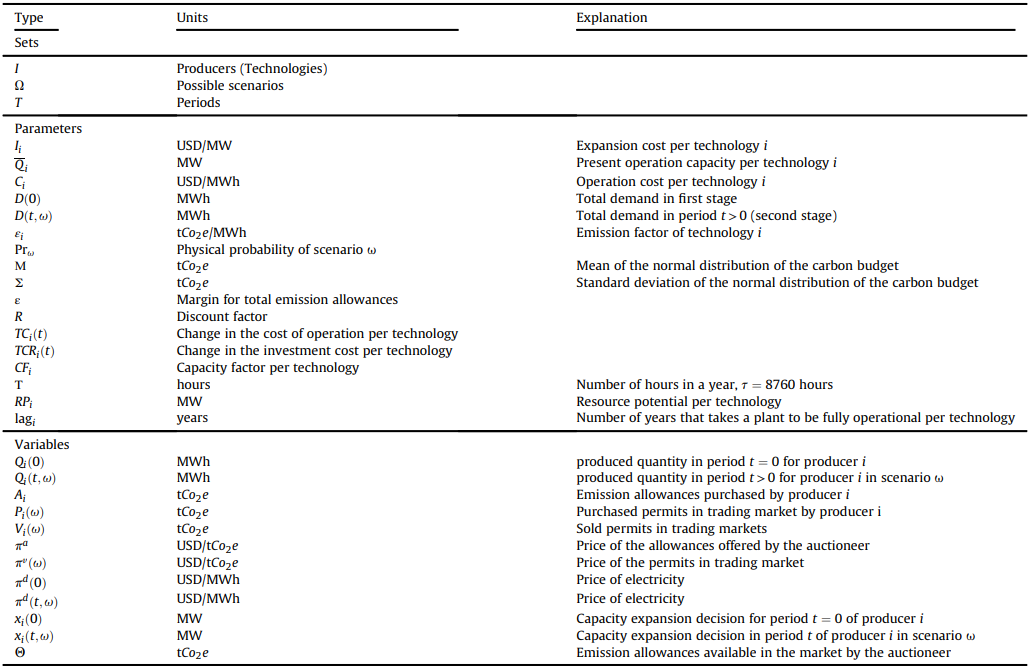
\includegraphics[width=15cm]{docs/DocumentoMemoria/core/images/Tabla amigo.png}
    \caption{Nomenclatura modelo original (Fuente: \protect\citeB{amigo_two_2021})}
    \label{fig:nomenclatura1}
\end{figure}

El modelo de \textit{cap and trade} propuesto se divide en dos partes que modelan el problema de los agentes (subastador y productores). Por una parte los agentes buscan maximizar sus beneficios (racionalidad individual) y, por otra parte, se definen condiciones de mercado que completan el problema de equilibrio (racionalidad social).
\vspace{2.5mm}

Por un lado, está el problema de los productores, mostrado en la ecuación \ref{fo:prod}. Este está acotado por restricciones de capacidad en generación en la restricción \ref{res:1}, restricción en generación inicial en \ref{res:2}, de límites en capacidad en \ref{res:3} y venta y compra de permisos en \ref{res:4} y \ref{res:5}. 

\begin{align}
\min_{(x_i,Q_i,A_i,P_i,V_i)\in \mathbb{X}} &  f_i \big( \pi^d(0),Q_i(0)\big)+ A_i \pi^{a} + I_i x_i(0) \nonumber \\ 
& + \sum_{\omega} Pr(\omega)   \Bigg[ \sum_{t>0} \frac{1}{(1+R)^t} \Big[ TC_i(t,\omega)\cdot f_i \big( \pi^d(t,\omega),Q_i(t,\omega) \big)  \nonumber \\
 & + TCR_i(t,\omega) \cdot I_i\cdot x_i(t,\omega) \Big] + \pi^v(\omega)\cdot \big(P_i(\omega)-V_i(\omega)\big) \Bigg]  \label{fo:prod}\\
     \textrm{s.t \ } \nonumber
\end{align}
\begin{align}
    \Big(CF_i \cdot\tau\Big)  \Bigg[\bar{Q}_i + \sum_{t^{\prime}<\bar{t}} x_i(t^\prime,\omega) + x_i(0)+ \bar{Q}_i(t) \Bigg] - Q_i(t,\omega) & \geq 0  & \forall  \quad i,\omega, t  > 0 & \quad (\alpha_{i,\omega,t})\label{res:1}\\
    \Big(CF_i\cdot\tau \Big)\bar{Q_i}-Q_{i}(0) & \geq 0  & \forall  \quad i & \quad (\kappa_i) \label{res:2}\\
     RP_i - \bar{Q}_i  - x_i(0) - \sum_{t > 0} x_i(t,\omega) & \geq 0 &  \forall \quad i,\omega &   \quad (\psi_{i,\omega}) \label{res:3}\\
 A_{i} -V_i(\omega) & \geq  0  & \forall  \quad \omega & \quad (\beta_{i,\omega}) \label{res:4}\\
 A_{i} + (P_i(\omega) - V_i(\omega))-\sum_{t>0}Q_i(t, \omega)\cdot \varepsilon_{i}-Q_i(0)\varepsilon_{i} & \geq  0  &\forall \quad \omega & \quad (\gamma_{i,\omega})\label{res:5}\\
 Q_i(0) & \geq  0 & \forall \quad i & \quad (\lambda_i) \label{res:q0}\\ 
 Q_i(t, \omega) & \geq  0   & \forall \quad \omega, t >0 & \quad (\delta_{i,\omega,t})\label{res:qt}\\
  x_i(0) & \geq  0 & \forall  \quad i & \quad (\xi_i)  \label{res:capi0}\\ 
  x_i(t, \omega) & \geq  0   & \forall  \quad \omega, t >0 & \quad (\varphi_{i,\omega,t})\label{res:capt}
  \end{align}

Es importante considerar que las variables presentes al final de cada restricción (por ejemplo $\varphi_{i,\omega,t}$ en la restricción \ref{res:capt}) corresponden a las variables duales de cada una, respectivamente.
\vspace{2.5mm}

Por otro lado, el problema del subastador está formulado de la siguiente forma en la función objetivo \ref{eq:sub}. En la sección siguiente, se explica con más detalle este modelo y sus restricciones.

\begin{equation}
\begin{array}{rrclcl}
    \displaystyle \min_{\theta} &-\theta \pi^a + F(\theta) \\\textrm{s.a.} \label{eq:sub}\\
\end{array}
\end{equation}
\begin{equation}
\begin{array}{cl}
    \varphi^-1 (\varepsilon )\sigma + \mu - \theta \geq 0 & (\eta) \label{res:sub1}
\end{array}
\end{equation}
\begin{equation}
\begin{array}{cl}
   \theta \geq 0 & (\varrho)\label{res:sub2}
\end{array}
\end{equation}

Con la finalidad de que ambos modelos se relacionen y puedan ser resueltos en un único sistema de ecuaciones como MCP, las variables de ambos problemas deben resolver las siguientes condiciones de mercado.

\begin{align}
   \sum_{i}A_i = \theta  &\quad (\pi^a)\label{rescom:1}
\end{align}

La anterior restringe que los permisos disponibles en el primer periodo no pueden superar los emitidos por el subastador.

\begin{align}
    \sum_{i}P_{i,\omega} = \sum_{i}V_{i,\omega} \quad& \forall \omega &(\pi^v (w))\label{rescom:2}
\end{align}
    


Esta explica que debe haber equilibrio en el mercado de compra y ventas de permisos.

\begin{align}
  \sum_{i}Q_i(0) = D(0) \quad (\pi^d (0))\label{rescom:3}  
\end{align}


La demanda energética debe ser abastecida en la primera etapa.

\begin{align}
    \sum_{i}Q_i(t,\omega) = D(t,\omega) \quad& \forall  \omega,t & (\pi^d (\omega,t))\label{rescom:4}
\end{align}

Finalmente, la restricción \ref{rescom:4} restringe que la demanda sea igual a la producción en todos los periodos y escenarios de la segunda etapa.
\vspace{2.5mm}

Al evaluar, en general, este modelo, el sistema permite a los generadores modificar sus sistemas en la segunda etapa con el propósito de obtener mayor utilidad al ajustar sus emisiones.
\vspace{2.5mm}

Esta oportunidad de reajuste otorga interesantes oportunidades, tanto a las empresas generadoras como al gobierno que pretende disminuir las emisiones. Por un lado, esta instancia permite a las empresas mejorar sus ganancias, acorde con las proyecciones de demanda. Por otro lado, el gobierno o ente regulador tendrá la opción de forzar ventas de permisos a las empresas de carbón para incentivar el cambio a opciones más renovables. 
\vspace{2.5mm}

Finalmente, el trabajo concluye que con el actual impuesto al carbono utilizado en Chile, no se llegaría al objetivo de eliminar el carbón como fuente de generación para el 2030 ni para ser carbono neutral en el año 2050. No obstante, proponen que definir un presupuesto de carbono (\textit{CAP}) entre 500-600 $MtCO_2 e$ o menos eliminaría al carbón en 15 años. También que con un \textit{CAP} menos severo (mayor $MtCO_2 e$) aumentaría la producción por energía con fuentes no convencionales(sustentables) a un 60-70\% del total de empresas generadoras, pero no eliminaría totalmente al carbón en el tiempo prometido. Como tercer punto, se concluye que si se añaden restricciones adicionales a las empresas generadoras (como imponer que estas deben vender sus permisos al llegar al año 2035), el objetivo de eliminar el carbón se puede alcanzar.
\vspace{2.5mm}

En el análisis anterior, se reconoce la importancia del subastador en este modelo y en el futuro de la generación eléctrica si se planea utilizar este sistema de \textit{cap and trade}. La cantidad de permisos emitidos según el \textit{CAP} deben estar de acuerdo con un criterio de optimalidad. Es decir, lo más cercanos a la realidad en cuanto al presupuesto determinado y la demanda futura. Por esto, se decide profundizar en el problema del subastador para que su rol en el sistema sea más real.
\vspace{2.5mm}

\section{Transformación del modelo original de Amigo et al. (2021) a un MCP}

Una de las maneras de resolver el modelo original de \citeB{amigo_two_2021}, gracias a su estructura, es transformarlo en un MCP. Esto es posible por medio del teorema de Karush-Kuhn-Tucker \ref{descripcionkkt} y sus condiciones resultantes. 
\vspace{2.5mm}

Por lo tanto, para lograr replicar el modelo original,  se debe realizar esta transformación. Es necesario entender que el modelo creado consiste de dos modelos que optimizan las utilidades de dos grupos de agentes distintos. Por un lado, se optimizan las utilidades de los productores de electricidad en el modelo \ref{fo:prod} y, por otro lado, está el modelo que optimiza al subastador o ente regulador de permisos de contaminación mostrado en \ref{eq:sub}. Con el fin de resolver el modelo como un solo problema MCP, es necesario agruparlos en un único problema de tipo MCP. Para lograr esto, además de encontrar las ecuaciones de KKT de cada uno de los grupos de agentes, es necesario incorporar las 4 condiciones de mercado \ref{rescom:1}, \ref{rescom:2},\ref{res:3},\ref{rescom:4} que relacionan ambos grupos de agentes.

\subsection{MCP problema del productor}\label{MCPproductor}

Primero, es necesario aplicar el teorema de KKT en el problema del productor \ref{fo:prod} para transformarlo en un MCP.
\vspace{2.5mm}

El lagrangeano del problema del productor se presenta de la siguiente manera: 

\begin{footnotesize}
\begin{align}
&\mathcal{L}_i(x_i,Q_i,A_i,P_i,V_i) = f_i \big( \pi^d(0),Q_i(0)\big)+ A_i \pi^{a} + I_i x_i(0)  +& \nonumber \\ 
&\sum_{\omega} Pr(\omega)\Bigg[ \sum_{t>0} \frac{1}{(1+R)^t} \Big[ TC_i(t)\cdot f_i \big( \pi^d(t,\omega),Q_i(t,\omega) \big) + TCR_i(t) \cdot I_i\cdot x_i(t,\omega) \Big] + \pi^v(\omega)\cdot \big(P_i(\omega)-V_i(\omega)\big) \Bigg]   + &\nonumber \\
&\kappa_{i}\Big[Q_i(0) -  \big(CF_i\cdot\tau \big)\bar{Q}_i \Big] +\sum_{\omega,t>0} \alpha_{i,\omega,t}\Bigg[Q_i(t,\omega) - \big(CF_i \cdot\tau\big) \big(\bar{Q}_i + \sum_{t^{\prime} \leq t } x_i(t,\omega) + x_i(0) \big)\Bigg] + & \nonumber \\ &\sum_{\omega}\beta_{i,\omega}\Big[V_i(\omega)-A_i \Big] + \sum_{\omega}\gamma_{i,\omega} \Big[-A_{i} - P_{i}(\omega) + V_i(\omega) +\sum_{t>0} Q_i(t,\omega) \varepsilon_{i} + Q_i(0)\varepsilon_{i}\Big] - \sum_{\omega, t>0}\delta_{i,\omega,t} Q_i(t,\omega) + & \nonumber \\ &\sum_{\omega}\psi_{i,\omega} \Big[  \bar{Q}_i+ x_i(0) + \sum_{t > 0} x_i(t,\omega) - RP_i \Big] - \lambda_{i}\Big[Q_{i}(0)\Big] - \sum_{\omega, t>0}\varphi_{i,\omega,t} x_i(t,\omega) - \xi_i x_i(0) & \label{eq:lagrange}
\end{align}
\end{footnotesize}

Al calcular las derivadas de primer orden, se obtienen:

\subsubsection{Derivada parcial respecto a $x_i(0)$}
\begin{footnotesize}
\begin{align}
    \frac{\partial \mathcal{L} }{\partial x_i(0)} = 0 = I_i  + \sum_{\omega}\psi_{i,\omega} -\sum_{\omega, t>0} \alpha_{i,\omega,t}(CF_i\cdot \tau) -\xi_i=0  \qquad \forall \  i \\
    \Leftrightarrow I_i  + \sum_{\omega}\psi_{i,\omega} -\sum_{\omega, t>0} \alpha_{i,\omega,t}(CF_i\cdot \tau) = \xi_i  \qquad \forall \  i 
\end{align}
\end{footnotesize}


En la que $\xi_i$ es la variable dual en \ref{res:capi0}. Por lo que esta KKT debe ser complementaria a $x_i(0)$, con lo que se obtiene la siguiente complementariedad:

\begin{footnotesize}
\begin{align}
    x_i(0)\geq 0 \qquad \forall \  i \\
    I_i  + \sum_{\omega}\psi_{i,\omega} -\sum_{\omega, t>0} \alpha_{i,\omega,t}(CF_i\cdot \tau) \geq 0  \qquad \forall \  i\\
    x_i(0)\cdot(I_i  + \sum_{\omega}\psi_{i,\omega} -\sum_{\omega, t>0} \alpha_{i,\omega,t}(CF_i\cdot \tau))=0 \qquad \forall \  i
\end{align}
\end{footnotesize}



\subsubsection{Derivada parcial respecto a $x_i(t,\omega)$}

\begin{footnotesize}
\begin{align}
    \frac{\partial \mathcal{L} }{\partial x_i(t,\omega)}= 0 = Pr(\omega) \Bigg[\frac{1}{(1+R)^t}TCR_i(t) \cdot I_i \Bigg] - \sum_{t> t\prime}\alpha_{i,\omega,t} ( CF_i \cdot \tau)+ \psi_{i,\omega}-\varphi_{i,\omega,t} \qquad  \forall \  i, \omega, t> 0\\
    \leftrightarrow Pr(\omega) \Bigg[\frac{1}{(1+R)^t}TCR_i(t) \cdot I_i \Bigg] - \sum_{t> t\prime}\alpha_{i,\omega,t} ( CF_i \cdot \tau)+ \psi_{i,\omega}=\varphi_{i,\omega,t} \qquad  \forall \  i, \omega, t> 0
\end{align}
\end{footnotesize}


En la que $\varphi$ es la variable dual en la restricción \ref{res:capt}, por lo que, para resolver como MCP, se tiene la siguiente complementariedad:


\begin{footnotesize}
\begin{align}
    Pr(\omega) \Bigg[\frac{1}{(1+R)^t}TCR_i(t) \cdot I_i \Bigg] - \sum_{t> t\prime}\alpha_{i,\omega,t} ( CF_i \cdot \tau)+ \psi_{i,\omega} \geq 0 \qquad  \forall \  i, \omega, t> 0\\
    x_i(t,\omega) \geq 0 \qquad  \forall \  i, \omega, t> 0\\
    (Pr(\omega) \Bigg[\frac{1}{(1+R)^t}TCR_i(t) \cdot I_i \Bigg] - \sum_{t> t\prime}\alpha_{i,\omega,t} ( CF_i \cdot \tau)+ \psi_{i,\omega})\cdot x_i(t,\omega)=0
\end{align}

\end{footnotesize}


\subsubsection{Derivada parcial respecto a $Q_i(0)$}
\begin{footnotesize}
\begin{align}
    \frac{\partial \mathcal{L} }{\partial Q_i(0)}= 0 =  \big(a_{i}+b_i Q_{i}(0)\big)-\pi^d(0) + \kappa_i  + \sum_{\omega} \gamma_{i,\omega}\varepsilon_i-\lambda_i \qquad \forall \  i  \\
     \leftrightarrow \big(a_{i}+b_i Q_{i}(0)\big)-\pi^d(0) + \kappa_i  + \sum_{\omega} \gamma_{i,\omega}\varepsilon_i = \lambda_i \qquad \forall \  i
\end{align}

\end{footnotesize}

$\lambda_i$ es la variable dual de la restricción \ref{res:q0}, por lo que, para resolver como MCP, se tiene lo siguiente:

\begin{footnotesize}
\begin{align}
    \big(a_{i}+b_i Q_{i}(0)\big)-\pi^d(0) + \kappa_i  + \sum_{\omega} \gamma_{i,\omega}\varepsilon_i \geq 0 \qquad \forall \  i  \\
    Q_i(0) \geq 0 \qquad \forall \  i  \\
    Q_i(0)\cdot ( \big(a_{i}+b_i Q_{i}(0)\big)-\pi^d(0) + \kappa_i  + \sum_{\omega} \gamma_{i,\omega}\varepsilon_i)=0 
\end{align}

\end{footnotesize}



\subsubsection{Derivada parcial respecto a $Q_i(t,\omega)$}
\begin{footnotesize}
\begin{align}
   \frac{\partial \mathcal{L} }{\partial Q_i(t,w)}= 
   0= Pr(\omega)  \frac{1}{(1+R)^t} \bigg( TC_i(t) \big(a_{i}+b_i Q_i(t,\omega)\big ) -\pi^d(t,\omega) \bigg) + \alpha_{i,\omega,\tau} + \gamma_{i,\omega} \varepsilon_{i} -\delta_{i,\omega,t} \qquad  \forall \ i, \omega, t > 0\\
   \leftrightarrow Pr(\omega)  \frac{1}{(1+R)^t} \bigg( TC_i(t) \big(a_{i}+b_i Q_i(t,\omega)\big ) -\pi^d(t,\omega) \bigg) + \alpha_{i,\omega,\tau} + \gamma_{i,\omega} \varepsilon_{i}= \delta_{i,\omega,t} \qquad \forall \ i, \omega, t > 0
\end{align}
\end{footnotesize}

$\delta_{i,\omega,t}$ es la variable dual de la restricción \ref{res:qt}, al resolverlo como MCP se tiene la siguiente complementariedad:

\begin{footnotesize}
\begin{align}
    Pr(\omega)  \frac{1}{(1+R)^t} \bigg( TC_i(t) \big(a_{i}+b_i Q_i(t,\omega)\big ) -\pi^d(t,\omega) \bigg) + \alpha_{i,\omega,\tau} + \gamma_{i,\omega} \varepsilon_{i} \geq 0 \qquad \forall \ i, \omega, t > 0\\
    Q_i(t,\omega) \geq 0 \qquad  \forall i, \omega, t > 0\\
    (Pr(\omega)  \frac{1}{(1+R)^t} \bigg( TC_i(t) \big(a_{i}+b_i Q_i(t,\omega)\big ) -\pi^d(t,\omega) \bigg) + \alpha_{i,\omega,\tau} + \gamma_{i,\omega} \varepsilon_{i})\cdot  Q_i(t,\omega)= 0 \qquad \forall \ i, \omega, t > 0
\end{align}

\end{footnotesize}


\subsubsection{Derivada parcial respecto a $A_i(t)$}
\begin{footnotesize}
\begin{align}
   \frac{\partial \mathcal{L} }{\partial A_i}= 0
   = \pi^{a} - \sum_{\omega}\beta_{i,\omega} - \sum_{\omega}\gamma_{i,\omega}  \qquad \forall \  i \\
\end{align}

\end{footnotesize}


Para resolverlo como MCP, se tiene la siguiente complementariedad:
\begin{footnotesize}
\begin{align}
    \pi^{a} - \sum_{\omega}\beta_{i,\omega} - \sum_{\omega}\gamma_{i,\omega} \geq 0 \qquad \forall  i\\
    A_i \geq 0 \qquad \forall  i\\
    (\pi^{a} - \sum_{\omega}\beta_{i,\omega} - \sum_{\omega}\gamma_{i,\omega}) \cdot A_i = 0 \qquad \forall  i
\end{align}

\end{footnotesize}


\subsubsection{Derivada parcial respecto a $V_i(w)$}
\begin{footnotesize}
\begin{align}
   \frac{\partial \mathcal{L} }{\partial V_i(w)}= 0
   = -Pr(\omega) \pi^v(\omega) + \beta_{i,\omega}  + \gamma_{i,\omega}  \qquad \forall \  i, \omega \\
\end{align}

\end{footnotesize}


Para resolverlo como MCP, se tiene la siguiente complementariedad:
\begin{footnotesize}
\begin{align}
    -Pr(\omega) \pi^v(\omega) + \beta_{i,\omega}  + \gamma_{i,\omega} \geq 0 \qquad \forall \  i, \omega \\
    V_i(w) \geq 0 \qquad \forall  i,\omega \\
    (-Pr(\omega) \pi^v(\omega) + \beta_{i,\omega}  + \gamma_{i,\omega}) \cdot  V_i(w) = 0  \qquad \forall \  i, \omega 
\end{align}

\end{footnotesize}


\subsubsection{Derivada parcial respecto a $P_i(w)$}
\begin{footnotesize}
\begin{align}
   \frac{\partial \mathcal{L} }{\partial P_i(w)}= 0
   = Pr(\omega) \pi^v(\omega) -\gamma_{i,\omega} \qquad \forall \  i, \omega \\
\end{align}

\end{footnotesize}


Para resolverlo como MCP, se tiene la siguiente complementariedad:
\begin{footnotesize}
\begin{align}
    Pr(\omega) \pi^v(\omega) -\gamma_{i,\omega} \geq 0 \qquad \forall \  i, \omega \\
    P_i(w) \geq 0 \qquad \forall  i,\omega \\
    (Pr(\omega) \pi^v(\omega) -\gamma_{i,\omega}) \cdot  P_i(w) = 0  \qquad \forall \  i, \omega 
\end{align}

\end{footnotesize}


\subsubsection{Completando el problema del productor}

Las demás complementariedades del problema del productor se producen al complementar las restricciones del modelo original con sus variables duales:

\begin{footnotesize}
\begin{align}
    & 0 \leq \big(CF_i \cdot \tau \big) \Bigg[\bar{Q}_i + \sum_{t\leq t^{\prime}} x_i(t,\omega) + x_i(0) \Bigg] - Q_i(t,\omega)  \perp \alpha_{i,\omega,\tau} \geq 0 \qquad \forall \ i, \omega, t  > 0\\
    & 0 \leq \Big(CF_i\cdot\tau \Big)\bar{Q}_i(0)-Q_{i}(0) \perp \kappa_i \geq 0 \qquad \forall \ i \\
    & 0 \leq  A_{i} - V_i(\omega) \perp \beta_{i,\omega} \geq 0 \qquad \forall  \ \omega \\
    & 0 \leq  A_{i} + P_{i} (\omega) - V_i(\omega) - \sum_{t>0} Q_i(t,\omega) \varepsilon_{i} -Q_i(0)\varepsilon_{i} \perp \gamma_{i,\omega} \geq 0 \qquad \forall \ i, \omega\\
    & 0 \leq  RP_i - \bar{Q}_i - x_i(0) - \sum_{t>0} x_i(t,\omega) \perp \psi_{i,\omega} \geq 0 \qquad \forall \ i,\omega 
\end{align}

\end{footnotesize}


\subsection{MCP problema del subastador}

Debido a que esta memoria se centra en la mejora e innovación de este modelo, este MCP se incluye en el siguiente capítulo ( \ref{MCP:subastador}). En él, luego de encontrar las restricciones, se proporciona una reestructuración del problema del subastador. 

\subsection{Condiciones de mercado}\label{MCPmercado}

Debido a que el modelo de \textit{cap and trade} funciona como un único sistema en el cuál los precios elegidos por el subastador influyen directamente en los generadores y la cantidad de permisos comprados por ellos afecta las ganancias del subastador, estos problemas deben ser resueltos en un solo modelo. Con el fin de lograr esto, los modelos del subastador y productor deben ser resueltos en un solo MCP que considere todas las variables y restricciones del sistema. Esta unión es posible al incluir las restricciones de condiciones de mercado \ref{rescom:1}, \ref{rescom:2},\ref{res:3},\ref{rescom:4}. A partir de estas, se calculan las siguientes complementariedades:

\subsubsection{Restricción de permisos disponibles}
\begin{footnotesize}
\begin{align}
 \pi^a \geq 0 \\
 \theta - \sum_{i}A_i = 0 \\
0 \leq \pi^a \perp \theta - \sum_{i}A_i= 0 \label{complementariedadcondicion1}
\end{align}
\end{footnotesize}


\subsubsection{Restricción de equilibrio en el mercado de compra y venta de permisos}

\begin{footnotesize}
\begin{align}
 \pi^v(\omega) \geq 0 \qquad \forall \omega\\
 \sum_{i}P_{i,\omega} - \sum_{i}V_{i,\omega} = 0 \qquad \forall \omega \\
0 \leq \pi^v(\omega) \perp \sum_{i}P_{i,\omega} - \sum_{i}V_{i,\omega} = 0 \qquad \forall \omega
\end{align}
\end{footnotesize}


\subsubsection{Abastecimiento de demanda en la primera etapa}

\begin{footnotesize}
\begin{align}
 \pi^d(0) \geq 0 \\
 \sum_{i}Q_i(0) - D(0) = 0\\
0 \leq \pi^d(0) \perp \sum_{i}Q_i(0) - D(0)= 0
\end{align}
\end{footnotesize}


\subsubsection{Abastecimiento de demanda en la segunda etapa}

\begin{footnotesize}
\begin{align}
 \pi^d(\omega,t) \geq 0 \qquad \forall \omega,t\\
 \sum_{i}Q_i(t,\omega) - D(t,\omega) = 0 \qquad \forall \omega,t\\
 0 \leq \pi^d(\omega,t) \perp \sum_{i}Q_i(t,\omega) - D(t,\omega) = 0 \qquad \forall \omega,t
\end{align}
\end{footnotesize}




\section{Costos de información y su aplicación en problemas de maximización de beneficios}\label{marco:costos}

En el contexto de modelos de optimización en economía, por ejemplo la maximización de utilidades, diversos factores pueden afectar su función objetivo. En varios casos, se reconoce la existencia de ``ruidos'' que afectan el rendimiento de una inversión. Estos modelos con ``ruidos'' pueden ser complejos de manejar ya que proveen predicciones estocásticas y no deterministicas \citeB{gabaix_behavioral_2019}. Además, se pueden interpretar como señales que afectan las decisiones de inversión. Estos pueden clasificarse como señales de información erróneas sobre la inversión que pueden afectar el rendimiento del inversionista. No obstante, se reconoce que en la realidad existe la posibilidad de gastar dinero en mejorar la información y, por ende, disminuir el ruido, gasto que se incluye en el modelo que se está evaluando.
\vspace{2.5mm}

La proporción de la información que está disponible, es definida en como información pública. Por ella no se debe pagar. Por lo tanto, si se quiere aumentar la información beneficiosa y disminuir el ruido, se incurre en un costo asociado para obtener esa información (por ejemplo, el costo de contratar servicios de consultoría financiera). \citeB{verrecchia_information_1982} fue de los primeros en explorar el incentivo de inversionistas de pagar para obtener información en los mercados financieros y mejorar sus inversiones. En otras palabras, demuestra que los agentes pagan para obtener mejor información y así obtener señales claras para disminuir el ruido. 
\vspace{2.5mm}

\citeB{gabaix_behavioral_2019} propone un modelo de optimización en el que se considera la precisión de la señal sujeta a su costo por mejorarla. En esta, se explica el costo de inatención que tienen las personas al tomar decisiones y su falta de representación en los modelos económicos.
\vspace{2.5mm}

Trabajos más contemporáneos proponen maneras de caracterizar la forma en que estos costos de información se presentan en la realidad. Por ejemplo, \citeB{dewan_estimating_2020} proponen la función objetivo del tomador de decisión de la siguiente forma: 

\begin{align}
    \max_{P}\quad rP-C(P)
\end{align}


En la que $P \in [0,1]$ representa el \textit{performance} (rendimiento en castellano) elegido por el tomador de decisión. A mayor rendimiento, más elevado será el total de \textit{reward} (premio en castellano) $r$ que el tomador obtendrá de la inversión o decisión tomada. $C(P)$ es el costo asociado con ese rendimiento. 
\vspace{2.5mm}

El modelado de este costo permite la resolución del problema del tomador de decisión. Este costo debe ser diferenciable\footnote{Una función diferenciable es aquella derivable por lo menos de primer orden} y bien comportado\footnote{\textit{well-behaved:} un costo continuo y convexo es bien comportado. \citeB{dewan_estimating_2020}}. Con esto, se llega a la \textbf{Proposición 4} del modelo de \citeB{dewan_estimating_2020} en que se demuestra que con el costo convexo, la función $\max_{P}\, rP-C(P)$ es cóncava. Por lo tanto, existe un máximo local que es también global máximo que resuelve el modelo.
\vspace{2.5mm}

 Estos autores consideran como ejemplo un costo $C(P)$ cuadrático, presentado en \ref{costocuad}, en el que $d \in [0,1]$ representa la información libre y gratis para todos (información pública) y $c$ el costo marginal de información. 

\begin{equation}
\begin{array}{rrclcl}
    {\mathcal{C}}(P)=\begin{cases}0,&P\leq d\\c(P-d)^2,&P>d\end{cases}\label{costocuad}\\
\end{array}
\end{equation}
\vspace{2.5mm}

\ref{costocuad} muestra que si el rendimiento es mayor a la información pública, se incurrirá un costo de obtención de un \textit{performance} mayor posible gracias a la obtención de información adicional.
\vspace{2.5mm}

Finalmente, al aplicar la \textbf{Proposición 4} se determina que el rendimiento óptimo, según el premio $r$ previamente definido, será dependiente de los costos asociados con información y su magnitud en comparación con el premio. Además, como se definió previamente, $P$ no puede superar a 1 ya que no se puede obtener un premio mayor al ofrecido.

\begin{equation}
\begin{array}{rrclcl}
    P^*(r) = \begin{cases}\frac{r}{2c}+d,&r\leq 2c(1-d)\\1,&r>2c(1-d)\end{cases}, \label{perforopt}\\
\end{array}
\end{equation}





